%===============================================================================
% Autoři: Michal Bidlo, Bohuslav Křena, Jaroslav Dytrych, Petr Veigend a Adam Herout 2018

\definecolor{mygreen}{rgb}{0.541,0.886,0.204}

\section{Úvod}
Disperze je všudypřítomný fyzikální jev jehož
dopady jsou pro nás často nežádoucí, ale
existuje i mnoho praktických aplikací, které
naopak tohoto jevu s~výhodou využívají.
Tato práce představuje konkrétně problematiku
disperze světla a přináší základní vhled do
fyzikální teorie za tímto jevem. Jsou zde
představeny
základní fyzikální zákony, kterými se disperze
světla řídí a tak je nutné poznamenat, že se
často jedná o~zjednodušený popis a mnohé
rovnice pouze hrubě aproximují skutečné
jevy. Cílem této práce ovšem nebyl detailní
rozbor tohoto fyzikálního jevu a zájemcům
o~hlubší vhled do této problematiky se tedy
doporučuje vyhledat odbornou literaturu.

\section{Disperze}
Na úvod je nutné poznamenat, že disperze jakožto
fyzikální jev je velmi široký pojem, který se netýká
pouze optiky a separace polychromatického světla
na jednotlivé složky v~důsledku rozdílných indexů lomu
je pouze jedním z~mnoha projevů disperze. Projevy
disperze je tedy možné pozorovat například i
u~mechanického nebo zvukového vlnění a nikoliv pouze
u~elektromagnetického vlnění či viditelného
světla. Tento text se ovšem ze zřejmých důvodů
zabývá pouze disperzí a jejími projevy u~světla.

\subsection{Disperze v~optice}
V~základní podobě se jedná jev, kdy \textit{fázová
rychlost} vlny závisí na její frekvenci, což nastává
pokud se vlna šíří v~takzvaném 
\textit{disperzním prostředí}. Pro jednoduché
monochromatické vlny by se mohlo
zdát, že nám tento jev nezpůsobí příliš mnoho
problémů. Jakmile ovšem začneme uvažovat například
o~přenosu informace pomocí obdélníkových pulzů,
zjistíme, že situace není zdaleka tak jednoduchá.
Dokonalé obdélníkové pulzy se totiž skládají
z~nekonečně mnoha harmonických složek o~různých
frekvencích, jak je možné
ukázat pomocí Fourierovy analýzy. Jev disperze
ovšem není limitován pouze na teoretické úvahy
a lze demonstrovat i na produkovatelných
nedokonalých obdélníkových pulzech, které se
skládají z~konečného počtu harmonických složek.

Efekt disperze u~takového pulzu je znázorněn na
obrázku~\ref{fig:square_wave_disp}, kde
\textit{transceiver} křivka odpovídá výchozí
podobě signálu u~zdroje a \textit{receiver}
křivka odpovídá signálu detekovanému u~přijímače
po průchodu disperzním médiem.
\begin{figure}[htbp]
    \centering
    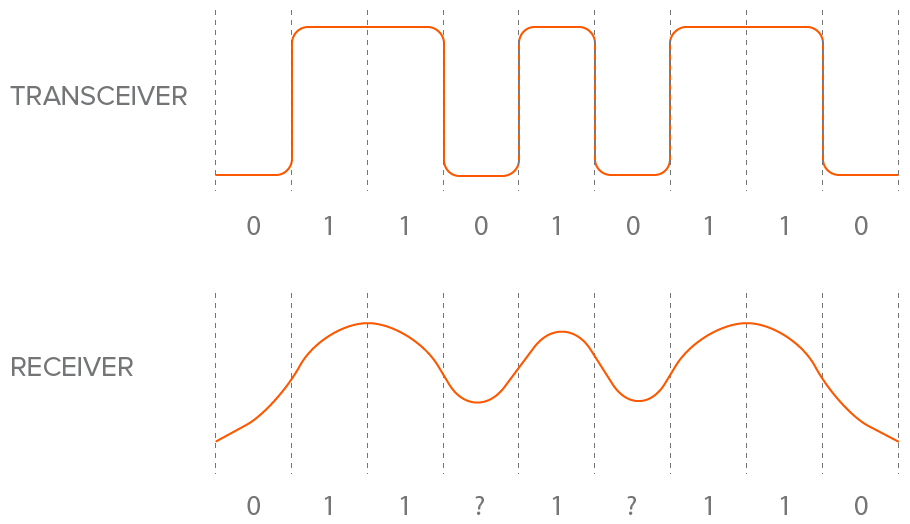
\includegraphics[scale=0.28]{img/BroadeningSignals.png}
    \caption{Znázornění disperzního jevu u~obdélníkových
    pulzů}
    \label{fig:square_wave_disp}
\end{figure}
Zde je možné pozorovat, že na straně přijímače
signál ztratil svůj původní tvar, konkrétně došlo
ke ztrátě vysokofrekvenčních změn v~signálu a
obdélníkové pulzy se rozprostřely v~čase. Důvodem
je právě skutečnost, že se pulzy skládají z~mnoha
harmonických složek o~různých frekvencích, které
médiem putují s~rozdílnými fázovými rychlostmi, což
se projevuje například tak, že složky s~vyššími
frekvencemi mají vyšší fázovou rychlost a
předbíhají tak původní pulz. Naproti tomu
složky s~nižšími frekvencemi mají nižší
fázovou rychlost a opožďují se tedy oproti
původnímu pulzu. Výsledkem je poté degradovaný
signál z~obrázku~\ref{fig:square_wave_disp},
kde došlo k~nežádoucímu rozprostření energie
v~čase. Konkrétní příklad postupné disperze
Gaussova pulzu v~čase je možné pozorovat \href{https://www.acs.psu.edu/drussell/Demos/Dispersion/dispersion.html}{zde}.

Nezbytnou podmínkou disperzního jevu je tedy
průchod disperzním médiem, jehož materiálové
charakteristiky způsobují disperzi.
Materiálovou disperzi můžeme popsat tzv.
\textit{disperzní závislostí}, na základě které
jsme schopni určit, jakou fázovou rychlost
budou mít jednotlivé složky o~různých frekvencích,
viz obrázek~\ref{fig:dispersion_rel}. Disperzní
závislost bude detailněji popsána v~následující
kapitole.
\begin{figure}[htbp]
\centering
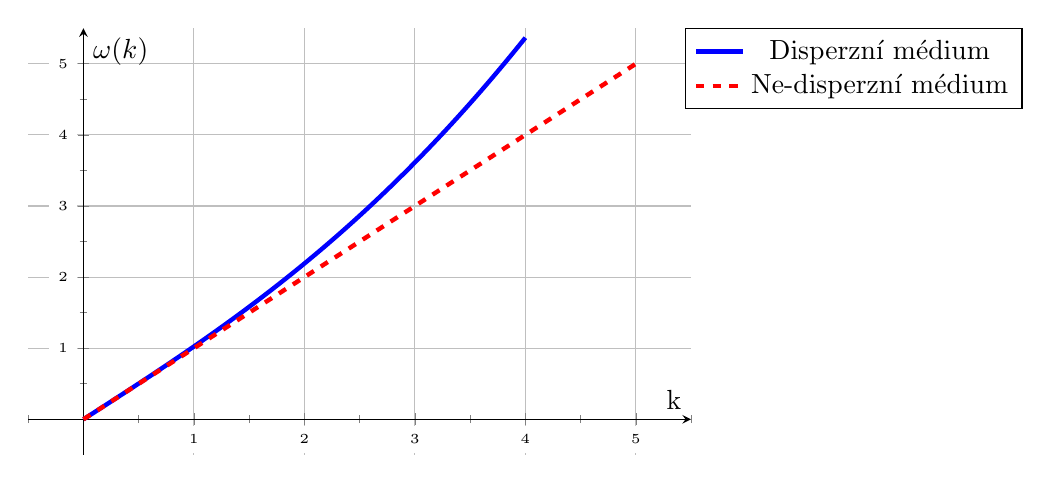
\begin{tikzpicture}
\begin{axis}[xmax=5,ymax=5,samples=500,grid=major,
xlabel={k},ylabel={$\omega(k)$}, width=10cm, height=7cm,
minor tick num=1,
grid=major,
axis lines=middle,
enlargelimits={abs=0.5},
ytick={0,1,...,5},
ticklabel style={font=\tiny,fill=white},
legend style={at={(1.5,1)}},
]

\addplot[blue, ultra thick, 
domain=0:4,
label=test,
mark=none,
samples=200,
unbounded coords=jump] {x * sqrt(1 + 0.05 * x^2)};

\addplot[red, ultra thick, 
domain=0:5,
dashed,
mark=none,
samples=200,
unbounded coords=jump] {x};

\addlegendentry{Disperzní médium}
\addlegendentry{Ne-disperzní médium}
\end{axis}
\end{tikzpicture}
\caption{Křivka disperzní závislosti
pro určení fázové rychlosti}
\label{fig:dispersion_rel}
\end{figure}

Často se také
materiálová disperze popisuje disperzní
křivkou, která určuje, jak se mění index
lomu materiálu na základě vlnové délky, viz
obrázek~\ref{fig:dispersion_curves}. Z~obrázku
je patrné, že pro různé materiály jsou křivky
odlišné, přičemž šedá oblast odpovídá viditelné
části spektra.
\begin{figure}[htbp]
    \centering
    \includesvg[scale=0.6]{img/dispersion_curves}
    \caption{Disperzní křivka udávající vztah
    mezi vlnovou délkou a indexem lomu materiálu}
    \label{fig:dispersion_curves}
\end{figure}

Kromě toho existuje i tzv. vlnovodová disperze,
se kterou se nejčastěji setkáme při práci
s~optickými vlákny a která k~celkové disperzi
přispívá nezanedbatelnou částí. Obecně se
vlnovodová disperze může projevit při šíření
vlny libovolným materiálem s~nehomogenní
strukturou, např. fotonickým krystalem, který
se dnes již také využívá v~optických
vláknech~\cite{ing_prace}. Běžně se ovšem
vlnovodová disperze odvíjí od geometrických
charakteristik vlákna, přesněji od poměru
mezi vlnovou délkou světla a poloměrem jádra
vlákna a také od profilu indexu lomu. Dle
citace: \uv{\textit{Tedy i za podmínek nulové
materiálové disperze je skupinové zpoždění
a konstanta šíření každého vidu funkcí vlnové
délky. Tento jev označujeme jako vlnovodovou
disperzi. Při přenosu nemonochromatického záření
přispívá ke zkreslení signálu stejným způsobem
jako disperze materiálová.}}~\cite{bc_prace}.
V~případě optických vláken je nutné brát v~potaz
mnoho dalších faktorů, které jsou ovšem mimo
rámec této práce. Pro představu dochází dále
k~tzv. vidové disperzi ve vícevidových vláknech,
která je způsobená rozdílnou délkou dráhy
každého vidu, což má za následek zkreslení
přenášeného signálu, jelikož energie každého
vidu dorazí na konec vlákna v~jiný časový okamžik,
viz obrázek~\ref{fig:modal_dispersion} pro lepší
představu.
\begin{figure}[htbp]
    \centering
    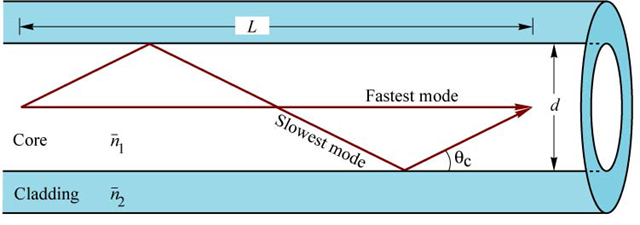
\includegraphics[scale=0.65]{img/modal_dispersion.png}
    \caption{Vidová disperze ve vícevidových optických
    vláknech}
    \label{fig:modal_dispersion}
\end{figure}

Jak je vidět, disperze má v~optice mnoho podob
a projevuje se různými způsoby, které nemusí
nutně souviset se separací složek světla
pomocí hranolu. Pro příklad, dříve zmíněná
vidová disperze nastavá i u~monochromatického
světla a nemá tedy nic společného s~chromatickou
disperzí, která nastává při lomu světla na optickém
hranolu.

\subsection{Disperzní médium a disperzní křivky}
Nejprve je nutné vysvětlit podstatu média bez
disperze a jak je možné na základě disperzní křivky
určit fázovou rychlost vlny, aby bylo později jasné,
jak, v~čem, a proč se disperzní médium liší.
Jako příklad média bez disperze lze uvést vakuum
pro elektromagnetické vlny~\cite{wiki_disp_rel}.
Typicky se také vzduch považuje za médium bez
disperze pro viditelné spektrum světla, což
však není tak úplně pravda. Ve skutečnosti i
vzduch způsobuje disperzi světla, která je ovšem
tak nepatrná, že dle~\cite{air_dispersive} není
za většiny běžných situací lidským okem viditelná.
Pro představu je na obrázku~\ref{fig:air_disp}
zobrazena křivka udávající index lomu vzduchu
podle konkrétní vlnové délky za určitých standardních
podmínek, viz~\cite{air_dispersive}.
\begin{figure}[htbp]
    \centering
    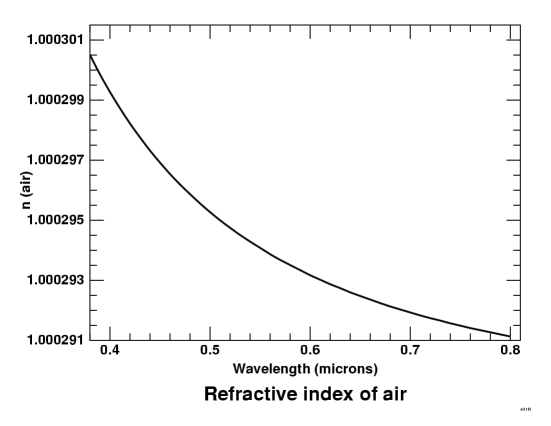
\includegraphics[scale=0.4]{img/disp_air.png}
    \caption{Disperzní křivka vzduchu}
    \label{fig:air_disp}
\end{figure}
Běžně se vzduch považuje za médium bez disperze
také pro zvukové vlny ve frekvenčním rozsahu,
který je slyšitelný lidským uchem. Nicméně vzduch
obsahuje molekuly $CO_2$ a je disperzní například
pro ultrazvuk~\cite{sound_dispersion}.

Obecně se disperzní závislost pro libovolný
fyzikální systém bez disperze získá vyřešením
následující vlnové rovnice, která ovšem popisuje
pouze situace, kdy máme jeden prostorový 
rozměr $x$:
$$
\frac{\partial^2 \psi}{\partial t^2}
   = c^2 \frac{\partial^2 \psi}{\partial x^2}.
$$
Člen $c \in \mathbb{R}$ je zde kladná konstanta,
která závisí na různých parametrech konkrétního
systému~\cite{wiki_wave_eq}. Řešením této rovnice
je libovolná funkce ve tvaru $f(x - ct)$, často
se ovšem řešení sestavují z~exponenciálních funkcí
následujícího tvaru:
$\psi(x,t) = Ae^{i(kx - \omega t)}$. Dosazením
exponenciální funkce tohoto tvaru do vlnové
rovnice získáme po úpravě následující triviální
disperzní závislost~\cite{harvard_disp}, která
odpovídá např. elektromagnetickým vlnám ve vakuu:
$$
\omega^2 = c^2k^2 \longrightarrow
\omega(k) = ck,
$$
kde $c$ je konstanta (nezávislá na $\omega$
i $k$) odpovídající
\textit{fázové rychlosti} vlny.
Triviální z~toho důvodu, že se jedná o~lineární
závislost, která odpovídá systému bez disperze,
jak uvidíme dále a jak je možné již vytušit
z~faktu, že $c$ je konstantní. Rychlost se nazývá
\textit{fázová}, abychom ji byli schopni odlišit
od \textit{grupové} rychlosti, kterou představíme
později, a také proto, že ve skutečnosti popisuje
jak rychle se u~sinusoidy $sin(kx - \omega t)$
pohybuje bod s~konstantní fází $kx - \omega t$.
Vztah pro fázovou rychlost je možné odvodit
následujícím způsobem:
$$
kx - \omega t = C \;\Longrightarrow\;
\frac{d(kx - \omega t)}{dt} = 0 \;\Longrightarrow\;
k\frac{dx}{dt} - \omega = 0 \;\Longrightarrow\;
\frac{dx}{dt} = \frac{\omega}{k} = v_f.
$$

Obrázek~\ref{fig:lin_disp_rel} obsahuje křivku
předchozí disperzní závislosti, která je lineární
a jedná se tedy o~přímku. Dále obrázek demonstruje,
že \textit{fázová} rychlost vlny graficky odpovídá
sklonu přímky procházející počátkem a konkrétním bodem
na přímce. Sklon přímky je dán její směrnicí, což
je v~tomto případě $c = \frac{\omega(k)}{k}$.
\begin{figure}[htbp]
\centering
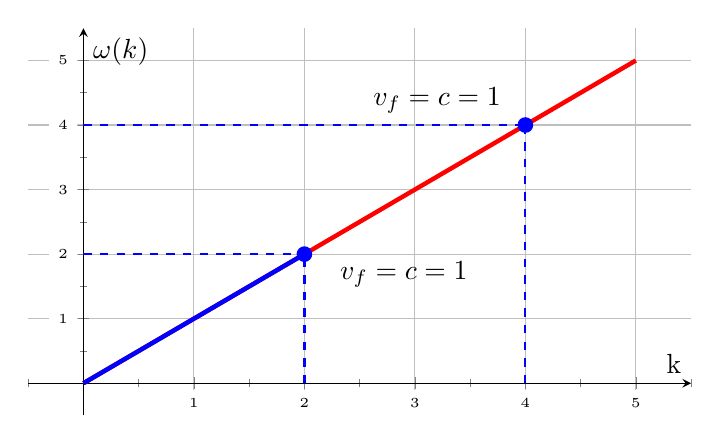
\begin{tikzpicture}
\begin{axis}[xmax=5,ymax=5,samples=500,grid=major,
xlabel={k},ylabel={$\omega(k)$}, width=10cm, height=6.5cm,
minor tick num=1,
grid=major,
axis lines=middle,
enlargelimits={abs=0.5},
ytick={0,1,...,5},
ticklabel style={font=\tiny,fill=white},
legend style={at={(1.5,1)}},
]

\addplot[red, ultra thick, 
domain=0:5,
mark=none,
samples=200,
unbounded coords=jump] {x};

\addplot[blue, thick, mark=none, dashed]
coordinates {(4, 0) (4, 4)};

\addplot[blue, thick, mark=none, dashed]
coordinates {(0, 4) (4, 4)};

\addplot[blue, thick, mark=none, dashed]
coordinates {(2, 0) (2, 2)};

\addplot[blue, thick, mark=none, dashed]
coordinates {(0, 2) (2, 2)};

\addplot[blue, ultra thick, mark=none]
coordinates {(0, 0) (2, 2)};

\node[
    label={[shift={(-0.8, -0.1)}]$v_f = c = 1$},
    circle,
    fill,
    inner sep=2pt,
    blue] at (axis cs:4,4) {};
    
\node[
    label={[shift={(0.9,-0.8)}]$v_f = c = 1$},
    circle,
    fill,
    inner sep=2pt,
    blue] at (axis cs:2,2) {};

%\addlegendentry{Ne-disperzní médium}
\end{axis}
\end{tikzpicture}
\caption{Lineární disperzní závislost $\omega(k) = ck$}
\label{fig:lin_disp_rel}
\end{figure}
Jak můžeme dále vidět, pro libovolný bod na této
křivce získáváme stejný poměr $\frac{\omega(k)}{k}$
a tedy i stejnou fázovou rychlost $v_f$, která je
konstantní a nezávislá na úhlové frekvenci či
vlnovém číslu. Zobrazená křivka tedy opravdu odpovídá
médiu bez disperze. Z~toho dále vyplývá, že ať
už máme jakkoliv složitý pulz (nebo vlnu), tak
\textit{fázová} rychlost libovolné
složky z~mnoha harmonických složek nám popisuje i
společnou rychlost celého pulzu a není tedy potřeba
zavádět nový druh rychlosti.

Problém ovšem nastává, pokud pracujeme se systémem,
který zahrnuje disperzi. Příkladem mohou být vlny
na tuhé struně, které popisuje následující vlnová
rovnice~\cite{yt_dispersion}:
$$
\frac{\partial^2 \psi}{\partial t^2}
   = \frac{T}{\mu} \cdot 
   \bigg(\frac{\partial^2 \psi}{\partial x^2} -
   \alpha \frac{\partial^4 \psi}{\partial x^4}
   \bigg),
$$
kde $T$ je síla napětí ve struně, $\mu$ je
hmotnost struny na jednotku délky a 
$\alpha \in \mathbb{R}$
je kladná konstanta odvíjející se od typu struny.
Řešením této vlnové rovnice je poté následující
vlnová funkce $\psi(x,t) = A\cos(kx - \omega t)$.
Po jejím dosazení do vlnové rovnice a dodatečných
úpravách získáváme tuto disperzní závislost:
$$
\omega^2 = \frac{T}{\mu}(k^2 + \alpha k^4)
\quad\longrightarrow\quad
\omega(k) = \sqrt{\frac{T}{\mu}} k 
\sqrt{1 + \alpha k^2}.
$$
Tato disperzní závislost je na první pohled
nelineární a její křivka pro konkrétní hodnoty
parametrů struny je zobrazena na
obrázku~\ref{fig:non_lin_disp_rel}.
\begin{figure}[htbp]
\centering
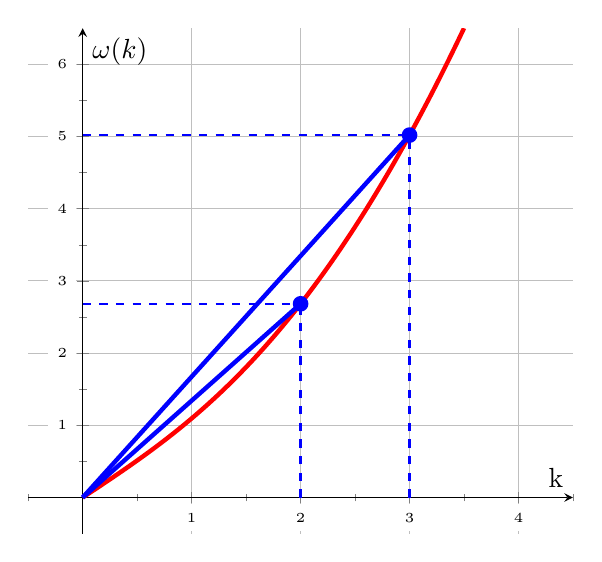
\begin{tikzpicture}
\begin{axis}[xmax=4,ymax=6,samples=500,grid=major,
xlabel={k},ylabel={$\omega(k)$}, width=8.5cm, height=8cm,
minor tick num=1,
grid=major,
axis lines=middle,
enlargelimits={abs=0.5},
ytick={0,1,...,6},
ticklabel style={font=\tiny,fill=white},
legend style={at={(1.5,1)}},
]

\addplot[red, ultra thick, 
domain=0:3.5,
mark=none,
samples=200,
unbounded coords=jump] {x * sqrt(1 + 0.2 * x^2)};

\addplot[blue, thick, mark=none, dashed]
coordinates {(3, 0) (3, {3 * sqrt(1 + 0.2 * 3^2)})};

\addplot[blue, thick, mark=none, dashed]
coordinates {(0, {3 * sqrt(1 + 0.2 * 3^2)}) 
(3, {3 * sqrt(1 + 0.2 * 3^2)})};

\addplot[blue, thick, mark=none, dashed]
coordinates {(2, 0) (2, {2 * sqrt(1 + 0.2 * 2^2)})};

\addplot[blue, thick, mark=none, dashed]
coordinates {(0, {2 * sqrt(1 + 0.2 * 2^2)}) 
(2, {2 * sqrt(1 + 0.2 * 2^2)})};

\addplot[blue, ultra thick, mark=none]
coordinates {(0, 0) (2, {2 * sqrt(1 + 0.2 * 2^2)})};

\addplot[blue, ultra thick, mark=none]
coordinates {(0, 0) (3, {3 * sqrt(1 + 0.2 * 3^2)})};

% \addplot[violet, ultra thick, mark=none]
% coordinates {(2, 0) (3, 0)};

% \addplot[violet, ultra thick, mark=none]
% coordinates {(0, {2 * sqrt(1 + 0.2 * 2^2)}) 
% (0, {3 * sqrt(1 + 0.2 * 3^2)})};

\node[
    circle,
    fill,
    inner sep=2pt,
    blue] at (axis cs:3,{3 * sqrt(1 + 0.2 * 3^2)}) {};
    
\node[
    circle,
    fill,
    inner sep=2pt,
    blue] at (axis cs:2,{2 * sqrt(1 + 0.2 * 2^2)}) {};

%\addlegendentry{Ne-disperzní médium}
\end{axis}
\end{tikzpicture}
\caption{Nelineární disperzní závislost $\omega(k) = 
\sqrt{\frac{T}{\mu}} k \sqrt{1 + \alpha k^2}$}
\label{fig:non_lin_disp_rel}
\end{figure}
Jak je vidět, pro různé body na křivce (různé
hodnoty úhlové frekvence) získáváme přímky
s~různými směrnicemi, což se graficky projeví
na sklonu přímky, který se pro každý bod na křivce
liší. Zároveň zde platí dříve odvozený vztah pro
lineární disperzní závislost a sklon přímky je
tedy opět roven \textit{fázové} rychlosti sinusoidy
s~danou frekvencí.

Otázkou ovšem je, zda je nyní možné nalézt nějakou
\uv{společnou} rychlost, která charakterizuje
vlnu s~dvěma a více harmonickými složkami, jestliže
se každá z~nich pohybuje vlastní rychlostí.
Odpověď je ano, přičemž tuto společnou rychlost
nazýváme \textit{grupovou}. Nyní si demonstrujeme,
jak je možné jednoduše odvodit vztah pro
grupovou rychlost složením pouhých dvou
sinusoid a jak je možné ji určit graficky
z~disperzní křivky. Uvažujme tedy, že máme
následující dvě vlny:
\begin{alignat*}{1}
\psi_1(x, t) &= A\cos(k_1x - \omega_1t)\\
\psi_2(x, t) &= A\cos(k_2x - \omega_2t)
\end{alignat*}
Jestliže tyto vlny složíme dohromady
s~využitím trigonometrického vzorečku:
$$
\cos \theta +\cos \varphi =2\cos \left({\frac {\theta +\varphi }{2}}\right)\cos \left({\frac {\theta -\varphi }{2}}\right),
$$
získáme následující složenou vlnu:
$$
\psi_1(x, t) + \psi_2(x, t) =
2A\cos\Big(\overline{k}x - \overline{\omega}t\Big)
\cos\Big(\frac{\Delta k}{2}x - 
\frac{\Delta\omega}{2}t\Big),
$$
kde $\overline{k} = \frac{k_1 + k_2}{2}$,
$\overline{\omega} = \frac{\omega_1 + \omega_2}{2}$,
$\Delta k = k_1 - k_2$ a 
$\Delta\omega = \omega_1 - \omega_2$.
Obrázek~\ref{fig:wave_sum} ukazuje prostorový
průběh této vlny s~parametry $k_1 = 10$ a
$k_2 = 8$ zachycený v~čase $t = 0$.
Z~obrázku je patrné, že výsledná vlna je
produktem dvou vln s~různými vlnovými
délkami, které jsou odlišné od původních
vlnových délek.
\begin{figure}[!ht]
\centering
\begin{minipage}{0.49\linewidth}
\centering
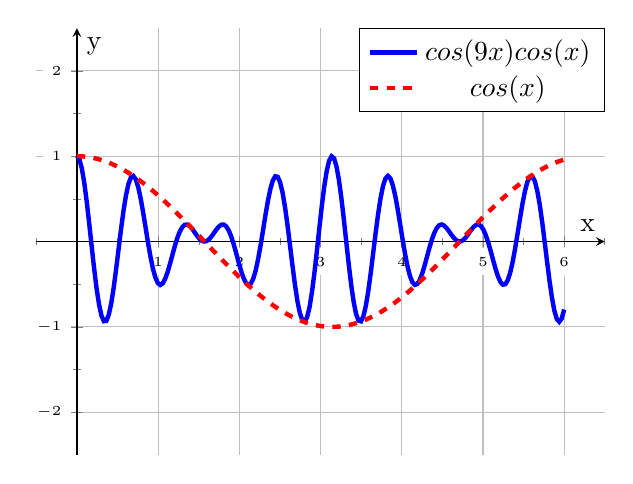
\begin{tikzpicture}
\begin{axis}[xmin=0, xmax=6, ymin=-2,
ymax=2,samples=500,grid=major,
xlabel={x},ylabel={y}, width=8.8cm, height=7cm,
minor tick num=1,
grid=major,
axis lines=middle,
enlargelimits={abs=0.5},
ytick={-2,-1,...,2},
ticklabel style={font=\tiny,fill=white},
legend style={at={(1,1)}},
]

\addplot[blue, ultra thick, 
domain=0:6,
mark=none,
samples=200,
unbounded coords=jump] {cos(deg(9*x)) *
cos(deg(-x))};

\addplot[red, ultra thick, dashed,
domain=0:6,
mark=none,
samples=200,
unbounded coords=jump] {cos(deg(x))};

\addlegendentry{$cos(9x)cos(x)$}
\addlegendentry{$cos(x)$}

\end{axis}
\end{tikzpicture}
\end{minipage}
\hfill
\begin{minipage}{0.49\linewidth}
\centering
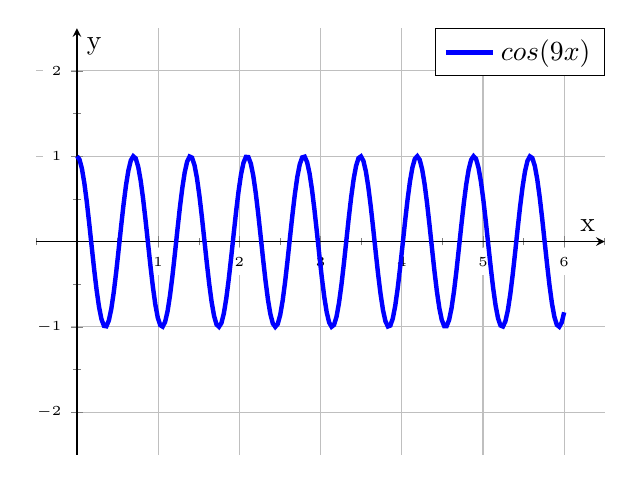
\begin{tikzpicture}
\begin{axis}[xmin=0, xmax=6, ymin=-2,
ymax=2,samples=500,grid=major,
xlabel={x},ylabel={y}, width=8.8cm, height=7cm,
minor tick num=1,
grid=major,
axis lines=middle,
enlargelimits={abs=0.5},
ytick={-2,-1,...,2},
ticklabel style={font=\tiny,fill=white},
legend style={at={(1,1)}},
]

\addplot[blue, ultra thick, 
domain=0:6,
mark=none,
samples=200,
unbounded coords=jump] {cos(deg(9*x))};

\addlegendentry{$cos(9x)$}

\end{axis}
\end{tikzpicture}
\end{minipage}
\caption{Moment složené vlny pro časový
okamžik $t = 0$}
\label{fig:wave_sum}
\end{figure}

Složka
$\cos\Big(\frac{\Delta k}{2}x - 
\frac{\Delta\omega}{2}t\Big)$
odpovídá červené, pomalu se měnící vlně.
Její rychlost šíření v~čase lze odvodit
stejným způsobem jako dříve pomocí obecného
vzorce pro rychlost šíření sinusoidy:
$$
\frac{dx}{dt} = \frac{\omega}{k} = v
\quad\longrightarrow\quad
v_1 = \frac{\frac{\Delta\omega}{2}}
{\frac{\Delta k}{2}} = 
\frac{\Delta\omega}{\Delta k}
$$
Pro tento konkrétní příklad lze rychlost $v_1$
označit za grupovou, přičemž k~obecnějšímu a
běžně používanému vztahu pro grupovou rychlost
se dopracujeme za chvíli. Červená vlna svým
způsobem provádí 
\uv{amplitudovou modulaci} a často se označuje
jako \textit{obálka} výsledné vlny. Naopak složka
$\cos\Big(\overline{k}x - \overline{\omega}t\Big)$
odpovídá modré, rychle se měnící vlně, kterou lze
pozorovat v~pravém grafu obrázku~\ref{fig:wave_sum}.
Její rychlost $v_2$ odvodíme stejným způsobem a
v~tomto konkrétním příkladu odpovídá fázové
rychlosti složené vlny:
$v_2 = \frac{\overline{\omega}}{\overline{k}}$.

Pokud bychom se na okamžik vrátili zpět
k~médiu bez disperze, tak můžeme na
obrázku~\ref{fig:wave_sum_non_dispersive}
pozorovat, že rychlost šíření obou složek
je konstantní a shodná s~původními fázovými
rychlostmi obou vln:
$$
v_{f1} = v_{f2} = \frac{\omega_1}{k_1} =
\frac{\omega_2}{k_2} = 
\frac{\overline{\omega}}{\overline{k}} = v_2 =
\frac{\Delta\omega}{\Delta k} = v_1.
$$
\begin{figure}[htbp]
\centering
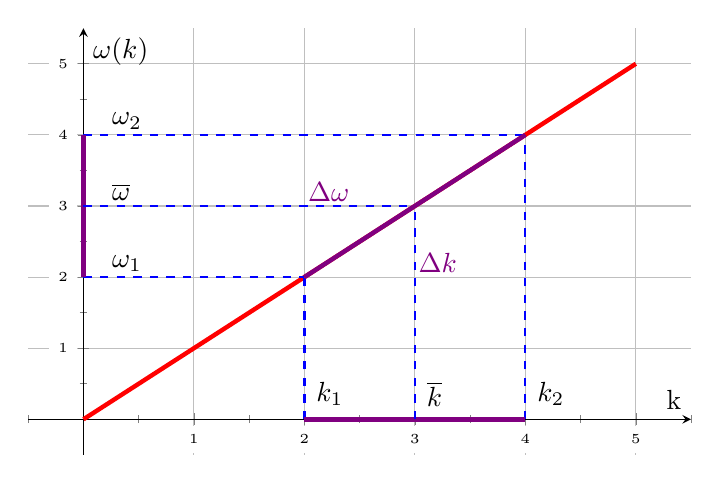
\begin{tikzpicture}
\begin{axis}[xmax=5,ymax=5,samples=500,grid=major,
xlabel={k},ylabel={$\omega(k)$}, width=10cm, height=7cm,
minor tick num=1,
grid=major,
axis lines=middle,
enlargelimits={abs=0.5},
ytick={0,1,...,5},
ticklabel style={font=\tiny,fill=white},
legend style={at={(1.5,1)}},
]

\addplot[red, ultra thick, 
domain=0:5,
mark=none,
samples=200,
unbounded coords=jump] {x};

\addplot[blue, thick, mark=none, dashed]
coordinates {(4, 0) (4, 4)};

\addplot[blue, thick, mark=none, dashed]
coordinates {(0, 4) (4, 4)};

\addplot[blue, thick, mark=none, dashed]
coordinates {(2, 0) (2, 2)};

\addplot[blue, thick, mark=none, dashed]
coordinates {(0, 2) (2, 2)};

\addplot[violet, ultra thick, mark=none]
coordinates {(2, 0) (4, 0)};

\addplot[violet, ultra thick, mark=none]
coordinates {(0, 2) (0, 4)};

\addplot[blue, thick, mark=none, dashed]
coordinates {(3, 0) (3, 3)};

\addplot[blue, thick, mark=none, dashed]
coordinates {(0, 3) (3, 3)};

\addplot[violet, ultra thick, mark=none]
coordinates {(2, 2) (4, 4)};
    
\node[
    label={
    [right,yshift=2.1ex,xshift=0.3em]180:
    {$\overline{k}$}},
    inner sep=2pt] at (axis cs:3,0) {};
    
\node[
    label={
    [right,yshift=2.1ex,xshift=0.3em]180:
    {$k_1$}},
    inner sep=2pt] at (axis cs:2,0) {};
    
\node[
    label={
    [right,yshift=2.1ex,xshift=0.3em]180:
    {$k_2$}},
    inner sep=2pt] at (axis cs:4,0) {};
    
\node[
    label={
    [right,yshift=0.5em,xshift=2.1ex]180:
    {$\overline{\omega}$}},
    inner sep=2pt] at (axis cs:0,3) {};
    
\node[
    label={
    [right,yshift=0.5em,xshift=2.1ex]180:
    {$\omega_1$}},
    inner sep=2pt] at (axis cs:0,2) {};
    
\node[
    label={
    [right,yshift=0.5em,xshift=2.1ex]180:
    {$\omega_2$}},
    inner sep=2pt] at (axis cs:0,4) {};
    
\node[
    label={
    [right, shift={(0,0.5em)}]180:
    {$\color{violet}\Delta\omega$}},
    inner sep=2pt] at (axis cs:2,3) {};
    
\node[
    label={
    [right, shift={(0,0.5em)}]180:
    {$\color{violet}\Delta k$}},
    inner sep=2pt] at (axis cs:3,2) {};

\end{axis}
\end{tikzpicture}
\caption{Fázová a grupová rychlost složené vlny
v~médiu bez disperze}
\label{fig:wave_sum_non_dispersive}
\end{figure}
To je opět dáno tím, že závislost je lineární
a poměr mezi průměrnými hodnotami pro rychlost
$v_2$ i mezi rozdíly pro rychlost $v_1$ je
totožný s~poměry mezi parametry původních vln
$\psi_1$ a $\psi_2$ což demonstruje
obrázek~\ref{fig:wave_sum_non_dispersive}.
Nyní uvažujme, že $k_1$ vlny $\psi_1$ je téměř
shodné s~$k_2$ vlny $\psi_2$, neboli 
$k_1 \approx k_2$, což znamená, že i
kruhové frekvence obou vln jsou téměř totožné
$\omega_1 \approx \omega_2$. Pak platí následující:
$$
\frac{k_1 + k_2}{2} \approx k_1 \approx k_2
\quad\land\quad
\frac{\omega_1 + \omega_2}{2}
\approx \omega_1 \approx \omega_2
\quad\longrightarrow\quad
v_2 =\frac{\overline{\omega}}{\overline{k}}
= \frac{\omega}{k} = v_{f1} = v_{f2}
$$
Tím jsme se dopracovali k~tomu, že
\textit{fázová} rychlost složené vlny
$v_2$ je v~podstatě shodná s~původními
fázovými rychlostmi vln $\psi_1$ a $\psi_2$.
Zajímavější je ovšem vztah pro rychlost
$v_1$. Pokud se $k_1$ limitně blíží ke
$k_2$, pak se $\Delta k$ limitně blíží
k~nule (to stejné platí i pro $\Delta\omega$)
a vzorec pro rychlost $v_2$ pak v~podstatě
odpovídá derivaci:
$$
\lim_{k_1\to k_2}\frac{\omega_1 - \omega_2}
{k_1 - k_2}
\quad\longrightarrow\quad
v_2 = \frac{\Delta\omega}{\Delta k} = 
\frac{d\omega}{dk} = v_g
$$
Derivace skutečně odpovídá obecnému vzorci
pro \textit{grupovou} rychlost a graficky
odpovídá sklonu (směrnici) tečny v~konkrétním
bodě disperzní křivky. Je tedy zřejmé, že pro
médium bez disperze je grupová rychlost sinusoidy
konstantní a shodná s~její fázovou rychlostí, což
ovšem neplatí pro disperzní médium viz
obrázek~\ref{fig:group_velocity}.
\begin{figure}[htbp]
\centering
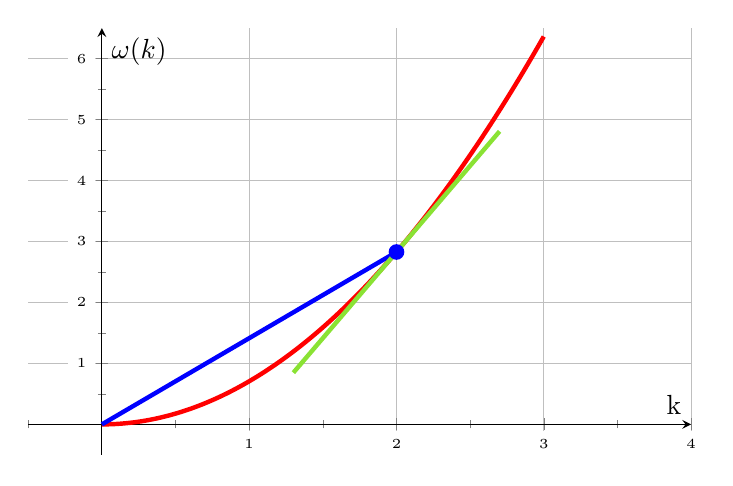
\begin{tikzpicture}
\begin{axis}[xmax=3.5,ymax=6,samples=500,grid=major,
xlabel={k},ylabel={$\omega(k)$}, width=10cm, 
height=7cm,
minor tick num=1,
grid=major,
axis lines=middle,
enlargelimits={abs=0.5},
ytick={0,1,...,6},
ticklabel style={font=\tiny,fill=white},
legend style={at={(1.5,1)}},
]

\addplot[red, ultra thick, 
domain=0:3,
mark=none,
samples=200,
unbounded coords=jump] {x * sqrt(0.5 * x^2)};

\addplot[blue, ultra thick, mark=none]
coordinates {(0, 0) (2, {2 * sqrt(0.5 * 2^2)})};

\addplot[mygreen, ultra thick,
domain=1.3:2.7,
mark=none,
samples=200,
unbounded coords=jump] {2.82842*x
- (2 * sqrt(0.5 * 2^2))};
    
\node[
    circle,
    fill,
    inner sep=2pt,
    blue] at (axis cs:2,{2 * sqrt(0.5 * 2^2)}) {};

\end{axis}
\end{tikzpicture}
\caption{Vizuální reprezentace fázové a grupové
rychlosti vlny pro disperzní médium}
\label{fig:group_velocity}
\end{figure}

Mohou tedy nastat tři různé situace, které
se v~našem jednoduchém příkladu s~dvěma vlnami
projeví následovně:
\begin{itemize}
    \item $\bm{v_g > v_f}$:
    \textit{anomální disperze}, která
    vzniká pokud máme \textit{konvexní}
    disperzní křivku. Jednoduše řečeno
    odpovídá situaci, kdy se rychlost
    šíření vlny v~médiu zvyšuje se
    zvyšující se frekvencí. Červená
    vlna z~obrázku~\ref{fig:wave_sum}
    tvořící obálku se v~tomto případě
    šíří v~čase rychleji než modrá
    vlna. Modrá vlna ovšem stále
    respektuje tvar obálky.
    
    \item $\bm{v_g = v_f}$:
    médium bez disperze, neboli lineární
    disperzní závislost. Obě složky se
v~čase šíří stejnou rychlosti.
    
    \item $\bm{v_g < v_f}$:
    \textit{normální disperze}, která
    vzniká pokud máme \textit{konkávní}
    disperzní křivku. Tato varianta odpovídá
    situaci, kdy se rychlost šíření vlny
    v~médiu snižuje se zvyšující se frekvencí.
    Modrá vlna se v~tomto případě propaguje
    obálkou vyšší rychlostí a respektuje její
    tvar.
\end{itemize}

Jednotlivé varianty lze pozorovat na
obrázku~\ref{fig:dispersion_types}.
Zajímavá je například situace, kdy je křivka
klesající, což znamená, že \textit{grupová}
rychlost je záporná. To se projeví tak, že
obálka (červená vlna) se v~čase šíří ve
směru záporné osy $x$, přičemž modrá vlna
se stále pohybuje v~kladném směru osy $x$,
jelikož její rychlost je kladná.
\begin{figure}[htbp]
\centering
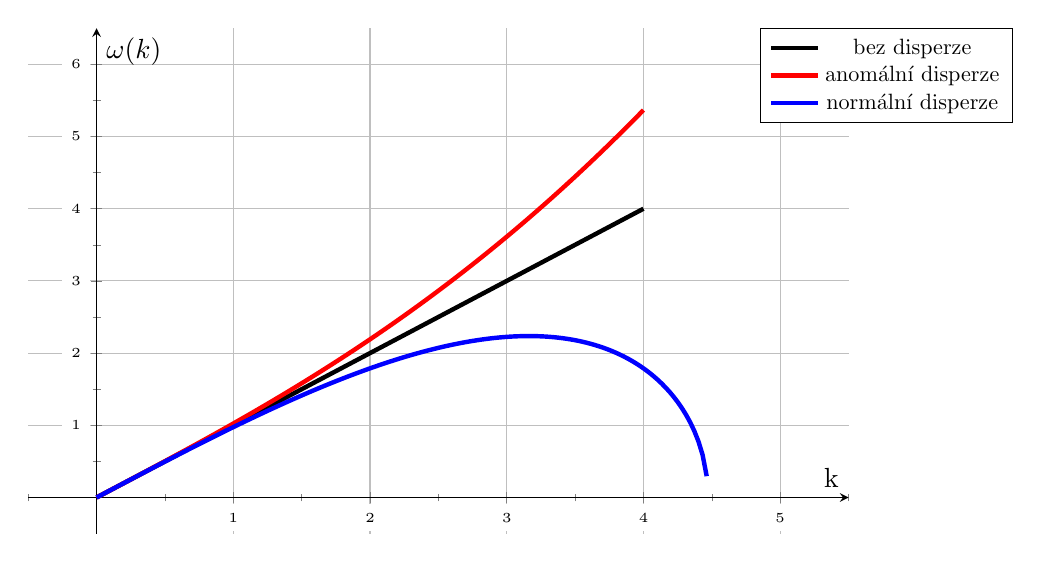
\begin{tikzpicture}
\begin{axis}[xmax=5,ymax=6,samples=500,grid=major,
xlabel={k},ylabel={$\omega(k)$}, width=12cm, 
height=8cm,
minor tick num=1,
grid=major,
axis lines=middle,
enlargelimits={abs=0.5},
ytick={0,1,...,6},
ticklabel style={font=\tiny,fill=white},
legend style={at={(1.20,1)},
nodes={scale=0.8, transform shape}}
]

\addplot[black, ultra thick,
domain=0:4,
mark=none,
samples=200,
unbounded coords=jump] {x};

\addplot[red, ultra thick, 
domain=0:4,
mark=none,
samples=200,
unbounded coords=jump] {x * sqrt(1 + 0.05 * x^2)};

\addplot[blue, ultra thick, 
domain=0:6,
mark=none,
samples=200,
unbounded coords=jump] {x * sqrt(1 - 0.05 * x^2)};

\addlegendentry{bez disperze}
\addlegendentry{anomální disperze}
\addlegendentry{normální disperze}

\end{axis}
\end{tikzpicture}
\caption{Typy disperze a jejich křivky}
\label{fig:dispersion_types}
\end{figure}
Tuto situaci
lze připodobnit ke známému tanečnímu pohybu
\textit{Moonwalk}, který proslavil Michael
Jackson, kdy je vytvořena iluze pohybu vpřed,
ovšem samotné tělo se stále pohybuje vzad.
Toto přirovnání je poměrně trefné, jelikož
v~praxi je právě \textit{grupová} rychlost to,
co nás zajímá, protože odpovídá rychlosti,
kterou se přenáší energie
vlněním~\cite{wiki_group_velocity} a tedy i
informace, pokud se bavíme například o~optických
kabelech. Grupová rychlost tedy nemůže být
větší než rychlost světla ve vakuu, na rozdíl
od fázové rychlosti, viz dále.

V~našem triviálním příkladu s~dvěma vlnami
bylo jednoznačné, pomocí které složky se
určí grupová rychlost. V~praxi se ovšem často
pracuje se složitějšími pulzy, které jsou tvořeny
složením mnoha harmonických složek a vyvstává
tak otázka, pro kterou frekvenci (vlnové číslo)
bychom měli vyhodnotit $v_g = \frac{d\omega}{k}$,
jelikož nejsme schopni nalézt jednu společnou
grupovou rychlost, jako tomu bylo možné v~našem
triviálním případě s~dvěma složkami.
Dle~\cite{harvard_disp} se často pro vyhodnocení
volí dominantní frekvence, kterou jsme schopni
nalézt pomocí Fourierovy transformace nad
daným pulzem.

Poslední zajímavostí je fakt, že při vhodné
disperzní závislosti je možné docílit toho,
že fázová rychlost vlny překročí rychlost
světla $c$. To nám ovšem nevadí, protože
ve skutečnosti nedochází k~přenosu energie
a není tak porušena teorie relativity. Aby
došlo k~přenosu energie, musíme způsobit změnu
ve vlně a každý takový signál se může šířit
pouze tak rychle jako čelní hrana této změny,
která již je limitována rychlostí světla.
Ve skutečnosti i grupová rychlost může ve
speciálních případech, jako je například
anomální disperze, překročit rychlost světla,
což nám ovšem opět nevadí, protože samotný
přenos energie tuto hranici nepřekročí.
Dokument~\cite{harvard_disp} poskytuje
detailnější popis této problematiky.


\subsection{Chromatická disperze}
Jedním z~nejznámějších projevů disperze je
separace jednotlivých složek polychromatického
světla pomocí hranolu z~vhodného disperzního
materiálu. Přesněji se jedná o~takzvanou
\textit{chromatickou} disperzi a separace světla
je pouze jejím důsledkem. Jak bylo ukázáno
v~předchozí kapitole, \textit{fázová} i
\textit{grupová} rychlost šíření vlny v~disperzním
prostředí je závislá na vlnové délce, případně
frekvenci vlny a můžeme tedy říci, že se ve
skutečnosti jedná o~funkce:
$v_p(\lambda)$, $v_g(\lambda)$. 
Tento fakt úzce souvisí s~vzorcem pro tzv.
\textit{absolutní} index lomu $n$, který udává poměr
mezi rychlostí šíření elektromagnetického vlnění ve
vakuu $c$ a rychlostí šíření v~libovolném jiném médiu $v$:
$n = \frac{c}{v}$.

Často se ovšem nespecifikuje,
že pro určení indexu lomu se využívá \textit{fázová}
rychlost vlny. Z~toho logicky vyplývá, že i
index lomu je pro disperzní média ve skutečnosti
funkcí vlnové délky a přesnější vzorec by tedy
mohl vypadat například následovně: 
$n(\lambda) = \frac{c}{v_p(\lambda)}$.
Pro lepší představu se často index lomu popisuje
jako koeficient udávající zpomalení oproti rychlosti
světla ve vakuu, pokud vyjádříme ze vzorce rychlost:
$v_p(\lambda) = \frac{c}{n(\lambda)}$. Index lomu
lze vyjádřit také pomocí poměru vlnových délek:
$n = \frac{\lambda_0}{\lambda}$, kde $\lambda_0$
je vlnová délka vlny ve vakuu a $\lambda$ je vlnová
délka v~daném médiu. Důležité je poznamenat, že při
přechodu z~jednoho média do druhého dochází ke změně
vlnové délky i rychlosti šíření tak, aby platil
vztah $v = \lambda f$, ale ke změně frekvence
vlnění \textit{nikdy} nedochází. To jsme schopni
pozorovat i prakticky, jelikož při lomu
monochromatického světla na hranolu nedochází ke
změně okem vnímané barvy, která je závislá právě
na frekvenci vlnění. Pro úplnost, vakuum má index
lomu roven $1$. Kromě klasického indexu lomu,
který je definován pro \textit{fázovou} rychlost
vlny, existuje i \textit{grupový index lomu}. Ten
je definován stejným způsobem jako klasický index
lomu, akorát pro \textit{grupovou} rychlost vlnění:
$n_g(\lambda) = \frac{c}{v_g(\lambda)}$.

V~minulé kapitole bylo zmíněno, že při vhodné
disperzní závislosti může fázová rychlost vlny
překonat rychlost světla, aniž by došlo k~porušení
teorie relativity, jelikož nedochází k~přenosu
informace. To ovšem znamená, že index lomu ve
skutečnosti může být nižší než $1$. Zajímavým
příkladem média s~takovým indexem lomu může být
ionosféra země, která je tvořena plazmatem.
Při vstupu vlny do takového média a refrakci
dochází k~odklonu vlnění od normály. 
Toho se využívá
například při rádiové komunikaci na velké
vzdálenosti~\cite{wiki_refractive_idx}.
Dokonce existují i materiály, jejichž index
lomu je záporný~\cite{wiki_negative_index}
a dochází tak k~negativní refrakci, se kterou
se běžně nesetkáváme.

Klíčové pro separaci barev ovšem je, že
index lomu ovlivňuje úhel lomu při přechodu
vlnění z~jednoho prostředí do druhého. Jelikož
index lomu závisí na vlnové délce, pak i samotný
uhel lomu je závislý na vlnové délce, což ve
výsledku způsobuje dříve zmíněnou a dobře známou
separaci bílého světla na jednotlivé složky při
průchodu hranolem pod vhodným úhlem. Opět je vhodné
zdůraznit, že \textit{disperzí} nazýváme konkrétně
závislost indexu lomu na vlnové délce a separace
složek světla je pouze jedním z~\textit{důsledků}
disperze. Dalším a tentokrát nepříjemným příkladem
důsledků disperze je závislost ohniskové vzdálenosti
čočky na vlnové délce. Tento jev je jedním z~typů
tzv. \textit{chromatické aberace}~\cite{wiki_aberration},
což je ve většině případů nežádoucí efekt, 
který se často musí různými způsoby (například i
pomocí software) alespoň částečně eliminovat.
Na obrázku~\ref{fig:aberration} můžeme pozorovat
praktický projev aberace, kdy jednotlivé barevné
složky měly při pořízení fotky posunuté ohniska, což
způsobilo rozostření a separaci barev na výsledné fotce.
\begin{figure}[htbp]
    \centering
    
\includegraphics[scale=0.20]{img/aberration.jpeg}
    \caption{Chromatická aberace v~praxi. Při
    pořízení fotky byly použity čočky zvýrazňující
    efekt aberace.}
    \label{fig:aberration}
\end{figure}

Jak konkrétně se světlo na rozhraní mezi prostředími
láme lze poté určit pomocí tzv. 
\textit{Snellova zákona}~\cite{wiki_snells_law}, 
který popisuje vztah mezi
úhlem dopadu a lomu při přechodu vlnění z~jednoho
prostředí s~indexem lomu $n_1$ do druhého prostředí
s~indexem lomu $n_2$. Konkrétně, pokud paprsek při
dopadu na rozhraní svírá s~normálou povrchu úhel
$\theta_1$, pak úhel $\theta_2$, který bude svírat
lomený paprsek lze vypočítat pomocí následujícího
Snellova zákona:
$$
\frac{\sin\theta_2}{\sin\theta_1} = \frac{v_2}{v_1}
= \frac{n_1}{n_2}
\quad\longrightarrow\quad
\theta_2 = \arcsin\Big(\frac{n_1}{n_2}\sin\theta_1\Big)
$$
Na obrázku~\ref{fig:snell_law} lze pozorovat situaci,
která nastane, pokud světlo přechází z~tzv. opticky
řidšího prostředí do opticky hustšího, což znamená,
že $n_2 > n_1$.
\begin{figure}[htbp]
    \centering
    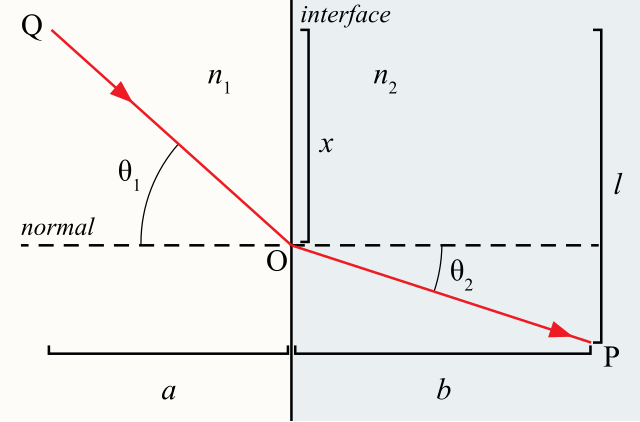
\includegraphics[scale=0.37]{img/snells_law.png}
    \caption{Přechod paprsku z~opticky řidšího
    prostředí do opticky hustšího. Úhel lomu
    $\theta_2$ lze vypočítat pomocí Snellova zákona.}
    \label{fig:snell_law}
\end{figure}
V~tomto případě se světlo láme směrem k~normále,
ale pokud bychom měli opačný případ, kdy $n_1 > n_2$,
pak by se světlo lámalo naopak směrem od normály.
Kromě toho nám Snellův zákon slouží také k~určení
tzv. úhlu totálního odrazu. Totální odraz je jev,
při kterém dochází k~odrazu veškerého dopadajícího
světla, pokud jsou splněny dvě podmínky:
\begin{enumerate}
    \item Vlnění přechází z~prostředí opticky
    hustšího do prostředí opticky řidšího,
    $n_1 > n_2$.
    
    \item Úhel, který dopadající paprsek svírá
    s~normálou je větší než tzv. \textit{kritický
    úhel} $\theta_c$
\end{enumerate}
Úplného odrazu se v~optice hojně využívá, zejména
v~optických kabelech, které by bez úplného odrazu
nemohly fungovat. Výpočet kritického úhlu $\theta_c$
je založen na principu, že Snellův zákon by v~některých
případech vyžadoval, aby sinus úhlu lomu byl 
větší než $1$, což samozřejmě není možné. V~takových
případech k~lomu nedochází a místo toho dochází
k~úplnému odrazu na rozhraní. Pro výpočet kritického
úhlu stačí spočítat hodnotu úhlu $\theta_1$,
pro kterou je úhel $\theta_2$ roven $90^\circ$:
$$
\theta_c = \arcsin\Big(\frac{n_2}{n_1}
\sin\theta_2\Big) = \arcsin\frac{n_2}{n_1},
$$
kde $\sin\theta_2 = \sin(90^\circ) = 1$.
Kritický úhel vlastně odpovídá největšímu možnému
úhlu dopadu, kdy ještě dojde k~lomu světla, přičemž
v~tomto případě se lomený paprsek šíří na rozhraní
obou prostředí. Obrázek~\ref{fig:critical_angle}
demonstruje tři možné situace, které mohou nastat.
\begin{figure}[htbp]
    \centering
    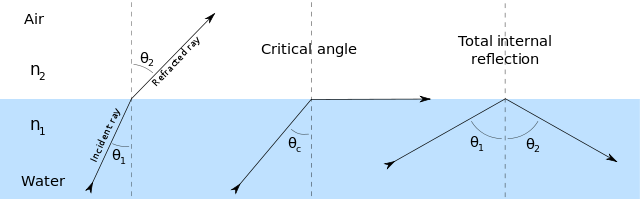
\includegraphics[scale=0.58]{img/critical_angle.png}
    \caption{Tři možné situace při přechodu světla
    z~opticky hustšího do opticky řidšího prostředí.}
    \label{fig:critical_angle}
\end{figure}

S~těmito znalostmi by již mělo být jasné, proč
dochází k~separaci barev bílého světla na hranolu
a jak můžeme jednoduše určit úhel lomu jednotlivých
barev.
\begin{figure}[htbp]
    \centering
    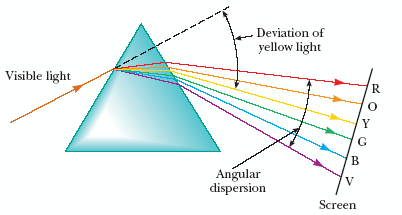
\includegraphics[scale=0.2]{img/prism.png}
    \caption{Separace bílého světla pomocí hranolu;
    znázornění \textit{úhlu deviace} a
    \textit{disperzního úhlu}, který svírá
    paprsek červeného světla s~paprskem
    fialového světla.}
    \label{fig:prism}
\end{figure}
Obrázek~\ref{fig:prism} ilustruje tuto situaci
a je vidět, že červené světlo s~největší vlnovou
délkou má nejvyšší úhel lomu (nejmenší úhel
deviace). Naopak fialové světlo s~nejmenší
vlnovou délkou má nejmenší úhel lomu (největší
úhel deviace). Jakým způsobem a jak moc se
světlo bude lámat opět záleží na konkrétním
materiálu a zda $n_1 > n_2$ nebo naopak.
U~běžných materiálů s~\textit{normální disperzí}
jako je sklo, se index lomu snižuje se zvyšující
se vlnovou délkou a úhel lomu se tím pádem
zvyšuje. Pokud bychom měli hranol z~materiálu
s~\textit{anomální disperzí}, pak by bylo pořadí
barev otočené.

Často potřebujeme znát \textit{úhel deviace}
paprsku,
případně \textit{disperzní úhel}, což je úhel,
který svírají paprsky s~extrémními úhly deviace
(minimální / maximální pro všechny obsažené
vlnové délky v~bílém světle),
v~našem případě červený a fialový paprsek na
obrázku~\ref{fig:prism}.
Vzorec pro úhel deviace lze odvodit na
základě geometrických vlastností hranolu,
trojúhelníku a čtyřúhelníku,
viz~\cite{ray_optics}[str. 331], kde je vzorec detailně
odvozen. Výsledný vzorec pro úhel deviace
$\delta$ vypadá následovně:
$\delta = i + e - \alpha$, kde $i$ je úhel
dopadu paprsku vstupujícího do hranolu,
$e$ je úhel lomu paprsku opouštějícího hranol
a $\alpha$ je vrcholový úhel hranolu.

Vrcholový úhel $\alpha$ i úhel dopadu $i$
známe, ale neznáme úhel lomu $e$, který je
potřeba vypočíst. Výpočet tohoto úhlu je
založený na jednoduchém trasování paprsku a využití
Snellova zákona. Obrázek~\ref{fig:prism_deviation}
demonstruje průchod červeného paprsku hranolem a
popisuje veškeré úhly, které jsou při výpočtu
potřeba. V~tomto případě platí $i = \theta_0$
a $e = \theta'_1$.
\begin{figure}[htbp]
    \centering
    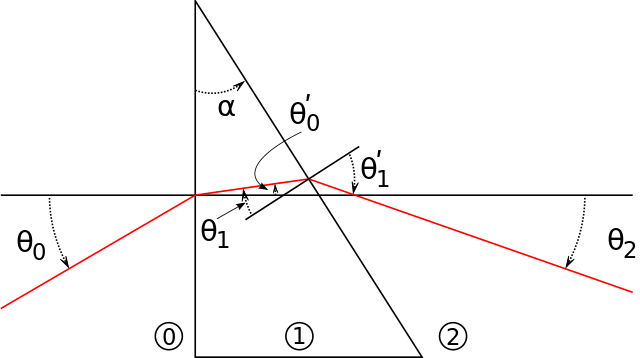
\includegraphics[scale=0.4]{img/prism_deviation.png}
    \caption{Refrakce paprsku při průchodu hranolem}
    \label{fig:prism_deviation}
\end{figure}
Paprsek nejprve dopadá na první rozhraní pod
úhlem $\theta_0$ a dochází k~refrakci. Úhel
$\theta'_0$ lomeného paprsku proto spočteme
následovně:
$$
\theta'_0 = \arcsin\Big(\frac{n_0}{n_1}
\sin\theta_0\Big),
$$
kde $n_0$ je index lomu média nalevo od hranolu
a $n_1$ je index lomu hranolu. Pomocí geometrie
se dále můžeme dopracovat k~následujícímu vzorci pro
druhý úhel dopadu $\theta_1 = \alpha - \theta'_0$.
Jakmile známe druhý úhel dopadu, můžeme opětovně
aplikovat Snellův zákon a získat druhý úhel lomu:
$$
\theta'_1 = \arcsin\Big(\frac{n_1}{n_2}
\sin\theta_1\Big).
$$
Výsledný úhel deviace $\delta$ je roven
součtu úhlů $\theta_0$ a $\theta_2$, kde
$\theta_2 = \theta'_1 - \alpha$, což odpovídá
obecnému vzorci $\delta = i + e - \alpha$.
Pro získání finálního vzorce tedy stačí
složit dohromady odvozené rovnice, přičemž pro
zjednodušení uvažujeme, že $n_0 = n_2$:
$$
\delta = \theta_0 + \theta_2 =
\theta_0 + \arcsin\Big(
\frac{n_1}{n_0}\sin\Big[
\alpha - \arcsin\Big(
\frac{n_0}{n_1}\sin\theta_0
\Big)\Big]\Big) - \alpha
$$

Důležité je uvědomit si, že indexy lomu použité
v~rovnicích jsou ve skutečnosti opět funkcemi
vlnové délky a zde byly pouze pro lepší čitelnost
zvoleny indexy lomu $n_0$, $n_1$ a $n_2$ pro
konkrétní vlnové délky. Konečně, pro určení
\textit{disperzního úhlu} pak stačí pouze odečíst
od největšího dosaženého úhlu deviace nejmenší
dosažený úhel deviace jak bylo zmíněno dříve,
tedy $\Phi = \delta_{max} - \delta_{max}$.
Na obrázku~\ref{fig:prism} se jedná o~úhly
deviace fialového a červeného paprsku, ale
v~obecném případě se jedná o~maximální a minimální
úhly, jelikož opět záleží na zvoleném materiálu,
který může způsobovat anomální disperzi.


\subsection{Využití disperze}
Přestože jsou projevy disperze v~mnoha
situacích, jako například u~optických vláken,
nežádoucí a je nutné je různými způsoby
zmírňovat či dokonce eliminovat, existuje
mnoho aplikací, pro které jsou projevy
disperze naopak klíčové.

Obecně se disperze využívá ve spektroskopii,
což je studium interakce mezi hmotou a
elektromagnetickým zářením~\cite{wiki_spectroscopy}.
Existují různé
druhy spektroskopie, které se odvíjí například
od toho, jaké části elektromagnetického spektra
se při experimentech využívají. Velmi důležitá
je potom tzv. infračervená (IR) spektroskopie,
která je klíčová zejména pro studium látek
v~organické chemii. Velmi zjednodušeně se využívá
toho, že molekuly absorbují určité frekvence
v~závislosti na tom, jaká je jejich struktura.
Typický spektroskopický experiment poté spočívá
v~systematickém ozařování daného studovaného
vzorku (látky) pomocí elektromagnetických vln
s~rozdílnými frekvencemi (souvisí s~energií
záření). Různé frekvence záření jsou poté
hmotou různě ovlivněny a dochází k~emisi
světla. Toto světlo je poté zachycováno na
detektoru, který produkuje tzv. emisní spektrum
jež se dále studuje.

Součástí detektoru je poté buď spektrometr
a nebo spektrograf, což jsou nástroje, které
přímo využívají disperzního jevu pro separaci
světla na jednotlivé složky o~různých frekvencích,
čímž produkují požadované spektrum. Dříve se
pro tyto účely využívalo jednoduchých optických
hranolů, které byly později nahrazeny tzv.
difrakčními mřížkami.

Technika spektroskopie je velmi rozmanitá a
má využití v~mnoha dalších odvětvích jako
například v~biomedicíně,
či astronomii při studiu složení hvězd, přičemž
na pozadí vždy v~nějaké podobě figuruje disperzní
jev. Dalo by se tedy říci, že spektroskopie
obecně je jednou z~hlavních aplikací disperzního
jevu.


\section{Demonstrační program}
Součástí tohoto semestrálního projektu
byla implementace programu, který vhodným
způsobem interaktivně demonstruje disperzní
jev a umožňuje uživateli experimentovat
s~různými parametry daného optického systému.
Konkrétně byla implementována vizualizace
chromatické disperze z~pohledu paprskové
optiky, jelikož se pravděpodobně jedná
o~nejznámější a nejnázornější projev disperze
světla v~optice.

Jádrem projektu je implementace algoritmu
sledování paprsku, který může procházet
různými optickými hranoly s~různými disperzními
vlastnostmi. Uživatel může manipulovat
s~počátkem či orientací jednotlivých paprsků
a nastavovat jejich vlnové délky. Dále
je možné manipulovat s~velikostí, pozicí
a rotací optických hranolů a
měnit body disperzní křivky materiálů
hranolů i prostředí.
Díky tomu lze nasimulovat jak normální,
tak anomální disperzi, vnější i vnitřní
úplný odraz a obecně i chování, které
běžné existující materiály nevykazují.
Index lomu mezi jednotlivými body disperzní
křivky je lineárně interpolován, což sice
neodpovídá žádnému reálnému materiálu,
nicméně pro účely demonstrace disperzního
jevu je snad dostačující.

Program je z~důvodu jednoduché přenositelnosti
implementován jako webová aplikace v~jazyce
\textit{JavaScript} s~využitím knihovny
\textit{PixiJS}, která slouží pro efektivní
vykreslování na \textit{HTML5} plátno s~využitím \textit{WebGL} API a grafické karty na pozadí.

\section{Záver}
V~rámci této práce byl nejprve obecně
představen disperzní jev a jeho nejčastější
projevy v~optice. Dále se text poměrně
detailně zabývá problematikou disperzních
médií a křivek, fázovou a grupovou rychlosti
a jejich spojitostí s~disperzí. Dále se
text zabývá konkrétně chromatickou
disperzí, Snellovým zákonem lomu a separací
polychromatického světla na optickém hranolu.
Závěr práce je věnován krátkému přehledu
praktických aplikací disperze v~různých vědních
oborech.
